\section{Drehstrom- Synchronmaschinen(DSM)}
    \subsection{Aufbau der DSM}
        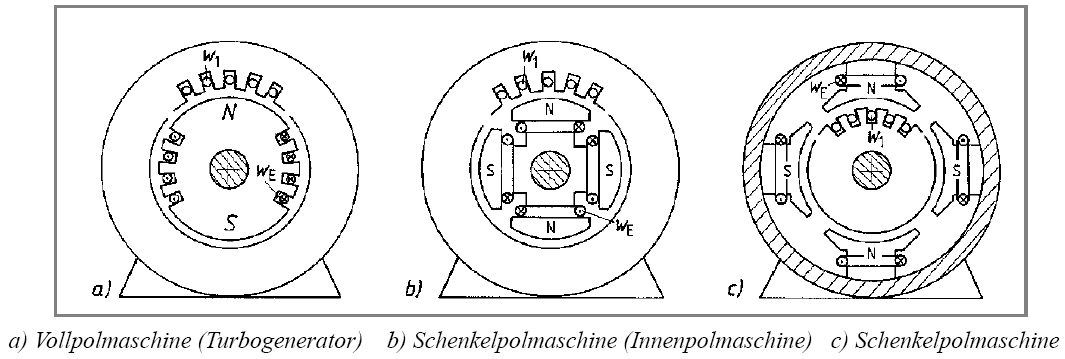
\includegraphics[width=12cm]{./images/Aufbau_DSM.png}\\
        \begin{description}
            \item[Innenpolmaschine:] Der Läufer ist ein Dauermagnet, oder wird mit Gleichstrom und über Schleifer
            zu einem solchem gemacht. Dieser läuft mit dem aussen anliegendem Drehfeld mit.
            \item[Aussenpolmaschine:] Der Läufer erzeugt ein Drehfeld, welches sich immer am konstanten Statorfeld
            ausrichtet. Worauf sich des Läufer dreht.
            \item[Turbomaschine:] Die Schleiferlose Variante. Mit Hilfe eines Hilfsgenerator auf der gleichen Welle
            wird ein Drehstrom erzeugt, welcher auf dem Läufer selbst gleichgerichtet wird. Damit wird dan ein
            konstantes Magnetfeld (Dauermagnet) erzeugt (wie die Innenpolmaschine).
        \end{description}
    \subsection{Ersatzschaltbild}
        \begin{minipage}{11cm}
            \abb{images/Ersatz_DSM.png}{8cm}{Ersatzschaltung DSM}    
            Es gibt 2 Unterteilungen: \\
            \begin{description}
                \item[Wirkleistung:] Gibt die DSM leistung ab oder nimmt sie auf. Zu erkennen ist das am Phasenwinkel
                zwischen $U_{KL}$ und $U_P$. Ist $U_P$ voreilend, so ist es ein \textbf{Generator}, anderseits ein
                \textbf{Motor}.
                \item[Blindleistung:] Blindleistung Auf- oder Abgabe. Bei \textbf{Übererregung} oder auch \textbf{kapazitiven
                Betrieb} gibt der DSM Blindleistung ab. Bei \textbf{Untererregung} oder auch \textbf{induktiven Betrieb}
                nimmt er auf.
            \end{description}
        \end{minipage}
        \begin{minipage}{8cm}
      %      \abb{images/Zeigerdiagram.png}{6cm}{Betriebszustände einer DSM}
    	  	\subsubsection{Phasenschieber}
	      	Ein DSG, der im Idealfall nur Blindleistung mit dem Netz austauscht. In der Praxis müssen die Verluste des DSG(Reibung, Ventilation, Stromwärme etc.) entweder vom Netz oder von einer Antriebsmaschine gedeckt werden.
			Der Phasenschieber kennt folgende Betriebsmodi:
     		\begin{itemize}
     			\item \textbf{\emph{übererregt}} $(U_p > U_N)$: der DSG gibt Blindleistung ab, verhält sich also bezüglich seiner Klemmen wie ein Kondensator.
      			\item \textbf{\emph{untererregt}} $(U_p > U_N)$: der DSG nimmt Blindleistung auf, verhält sich also bezüglich seiner Klemmen wie eine Induktivität.
      		\end{itemize}
        \end{minipage}
        \\ \\ \\  
        \begin{tabular}{|l|l|l|}
        \hline
       	& Übererregung & Untererregung \\ 
         \hline
        Motor & & \\
        &
        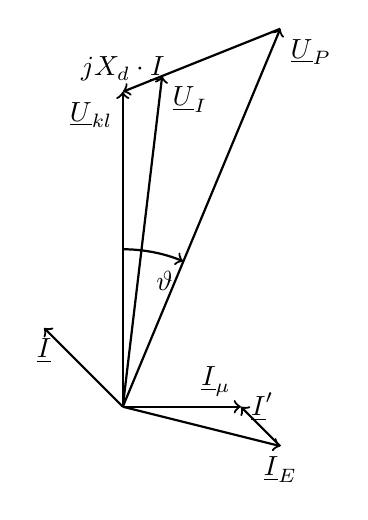
\begin{tikzpicture}[->,thick]
\coordinate (null) at (0,0) {};
\coordinate (I) at (-1,1) {};
\coordinate (Ukl) at (0,4) {};
\coordinate (Up) at (2,4.8) {};
\coordinate (Ie) at (2,-0.5) {};
\coordinate (Iu) at (1.5,0) {};

\draw (null) -- (I) node [anchor=north] {$\underline{I}$};

\draw (null) -- (Ukl) node [anchor=north east] {$\underline{U}_{kl}$};
\draw (null) -- (0.5,4.2) node [anchor=north west] {$\underline{U}_I$};
\draw (null) -- (Up) node [anchor=north west] {$\underline{U}_P$};
\draw (Up) -- (Ukl) node [anchor=south] {$jX_d\cdot\underline{I}$};

\draw (null) -- (Ie) node [anchor=north] {$\underline{I}_E$};
\draw (Ie) -- (Iu) node [anchor=west] {$\underline{I}^\prime$};
\draw (null) -- (Iu) node [anchor=south east] {$\underline{I}_\mu$};

\draw (0,2) arc [radius=2, start angle=90, delta angle=-22.5] node [anchor=north east] {$\vartheta$};
\end{tikzpicture} &
        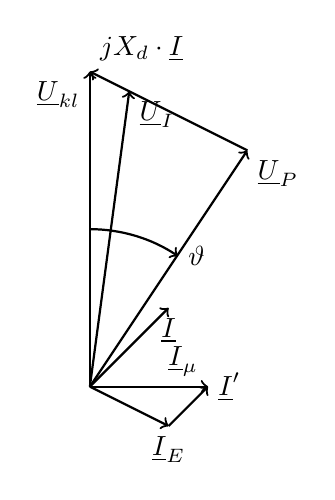
\begin{tikzpicture}[->,thick]
\coordinate (null) at (0,0) {};
\coordinate (I) at (1,1) {};
\coordinate (Ukl) at (0,4) {};
\coordinate (Up) at (2,3) {};
\coordinate (Ie) at (1,-0.5) {};
\coordinate (Iu) at (1.5,0) {};

\draw (null) -- (I) node [anchor=north] {$\underline{I}$};

\draw (null) -- (Ukl) node [anchor=north east] {$\underline{U}_{kl}$};
\draw (null) -- (0.5,3.75) node [anchor=north west] {$\underline{U}_I$};
\draw (null) -- (Up) node [anchor=north west] {$\underline{U}_P$};
\draw (Up) -- (Ukl) node [anchor=south west] {$jX_d\cdot\underline{I}$};

\draw (null) -- (Ie) node [anchor=north] {$\underline{I}_E$};
\draw (Ie) -- (Iu) node [anchor=west] {$\underline{I}^\prime$};
\draw (null) -- (Iu) node [anchor=south east] {$\underline{I}_\mu$};

\draw (0,2) arc [radius=2, start angle=90, delta angle=-34] node [anchor=west] {$\vartheta$};
\end{tikzpicture}\\
        \hline
         Generator & & \\
        &
         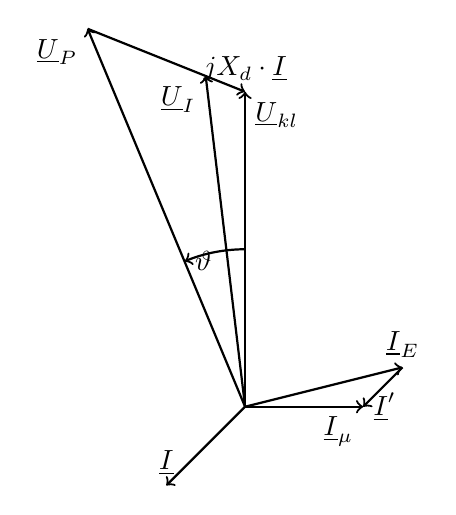
\begin{tikzpicture}[->,thick]
\coordinate (null) at (0,0) {};
\coordinate (I) at (-1,-1) {};
\coordinate (Ukl) at (0,4) {};
\coordinate (Up) at (-2,4.8) {};
\coordinate (Ie) at (2,0.5) {};
\coordinate (Iu) at (1.5,0) {};

\draw (null) -- (I) node [anchor=south] {$\underline{I}$};

\draw (null) -- (Ukl) node [anchor=north west] {$\underline{U}_{kl}$};
\draw (null) -- (-0.5,4.2) node [anchor=north east] {$\underline{U}_I$};
\draw (null) -- (Up) node [anchor=north east] {$\underline{U}_P$};
\draw (Up) -- (Ukl) node [anchor=south] {$jX_d\cdot\underline{I}$};

\draw (null) -- (Ie) node [anchor=south] {$\underline{I}_E$};
\draw (Ie) -- (Iu) node [anchor=west] {$\underline{I}^\prime$};
\draw (null) -- (Iu) node [anchor=north east] {$\underline{I}_\mu$};

\draw (0,2) arc [radius=2, start angle=90, delta angle=22.5] node [anchor=west] {$\vartheta$};
\end{tikzpicture} &
         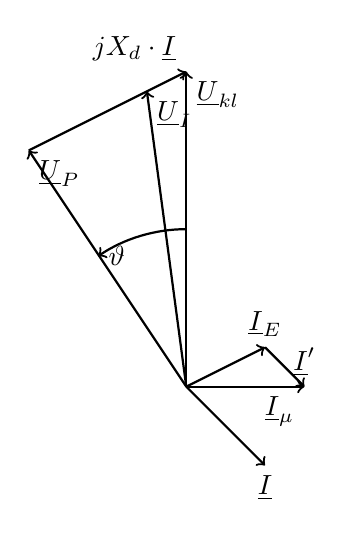
\begin{tikzpicture}[->,thick]
\coordinate (null) at (0,0) {};
\coordinate (I) at (1,-1) {};
\coordinate (Ukl) at (0,4) {};
\coordinate (Up) at (-2,3) {};
\coordinate (Ie) at (1,0.5) {};
\coordinate (Iu) at (1.5,0) {};

\draw (null) -- (I) node [anchor=north] {$\underline{I}$};

\draw (null) -- (Ukl) node [anchor=north west] {$\underline{U}_{kl}$};
\draw (null) -- (-0.5,3.75) node [anchor=north west] {$\underline{U}_I$};
\draw (null) -- (Up) node [anchor=north west] {$\underline{U}_P$};
\draw (Up) -- (Ukl) node [anchor=south east] {$jX_d\cdot\underline{I}$};

\draw (null) -- (Ie) node [anchor=south] {$\underline{I}_E$};
\draw (Ie) -- (Iu) node [anchor=south] {$\underline{I}^\prime$};
\draw (null) -- (Iu) node [anchor=north east] {$\underline{I}_\mu$};

\draw (0,2) arc [radius=2, start angle=90, delta angle=34] node [anchor=west] {$\vartheta$};
\end{tikzpicture}\\
         \hline
         \end{tabular}
        \renewcommand{\arraystretch}{1.4}
    \subsection{Allgemeine Formeln}
    \begin{tabular}[c]{ | p{6.5cm} | p{11.5cm} |}
    	\hline
    	Polpaarzahl	& $p$\\
    	\hline
    	Drehfeldzahl $[s^{-1}]$ bzw $[min^{-1}]$ & $n_d=\frac{f}{p}$ bzw
    	$n_d=\frac{f\cdot 60}{p}$\\
    	\hline
    	Schlupf $[-]$ & $s=\frac{n_d-n}{n_d}$\\
    	\hline
    	Spannungsfall über Synchroner Reaktanz & $U_{XD}=jX_d\cdot\underline{I}$
    	\\
    	\hline
    	Leerlauferregerstrom für Nennspannung & $I_{E0N}$\\
    	\hline
    	Lastabhängiger Erregerstrom & $\frac{I_E}{I_{E0N}}=\frac{U_p}{U_{Kl}}$\\
    	\hline
    	Klemmenspannung & $U_{kl} = \frac{U_N}{\sqrt{3}}$\\
    	\hline
    	Strang- bzw. Phasenspannung &
    	$\underline{U}_{kl}=\underline{U}_p+\underline{U}_{XD}$\\
    	\hline
    	Polradspannung & $U_p=\sqrt{U_{Kl}^2+X_d^2\cdot I^2+2\cdot U_{Kl}\cdot
    	X_d \cdot I\cdot sin \varphi}$\\
    	\hline
    	\multirow{2}{6.5cm}{Elekrischer Lastwinkel oder Polradwinkel  gem. ESB} & $\vartheta = arg(U_p)$ (Winkel zwischen $U_{p}$ und $U_{kl}$)\\ & $|U_P| \cdot sin(\theta) = |U_{XD}| \cdot cos(\Phi)$\\
    	\hline
    	Wirkleistung des DSG & $P_{el}=3\cdot
    	U_{Kl}\cdot\frac{U_p}{X_d}\cdot \sin\vartheta = 3 \cdot U_{Kl} \cdot I \cdot \cos{\varphi}$\\
    	\hline
    	Wirkkomponente des Statorstroms & $I \cdot \cos{\varphi} = \frac{U_p}{X_d} \cdot \sin{\varphi}$ \\
    	\hline
    	Antriebsmoment des DSG & $\begin{aligned}
    								M_{Welle} 	&=\frac{3\cdot60}{2\pi\cdot n \cdot
    								    				\eta}\cdot U_{Kl}\cdot\frac{U_p}{X_d}\cdot\sin\vartheta
    								    		&= \frac{3\cdot60}{2\pi\cdot n \cdot
    								    	    	\eta}\cdot U_{Kl}\cdot I \cdot \cos{\varphi}= \frac{P_{mech}}{\omega} \\
    								    	    &= \frac{\sqrt{3} \cdot U_N \cdot I_N \cdot cos\varphi_N \cdot p}{\eta \cdot 2 \cdot \pi \cdot f_N} 
    								\end{aligned}$\\
    	\hline
    \end{tabular}
    
    \subsection{Inselnetz}
    \begin{tabular}{|p{7cm}|p{11cm}|}
    		\hline
        	Netzstrom Generator & Verbraucherstrom vom Netz mit Immaginiärteil negiert !\\  
        	\hline
        	Zuleitungstrom Generator & Netzstrom mit Winkel $+ 180$\textdegree \\
        	\hline
        	Verbraucher induktiv & Generator kapazitiv $=$ übererregt \\
        	Verbraucher kapazitiv & Generator induktiv $=$ untererregt \\
        	\hline
        	Polradspannung & $\underline{U}_p = \underline{U}_{kl} - \underline{U}_{XD} $ \\
        	\hline
        	Polradspannung im Inselnetz & $U_p=\sqrt{U_{Kl}^2+X_d^2} $\\
        	\hline
        	Klemmenspannung & Y = 230V $\Delta$ = 400V \\
        	\hline
        	Klemmenspannung nach Lastabwurf & $U_{Kl} = \sqrt{3} \cdot U_p $\\
        	\hline
    \end{tabular}

    \subsection{Betriebsverhalten}
    	Siehe Abbildung \ref{fig:betriebsverhalten}
    	\begin{figure}[h!]
	    	\centering
	    	\begin{subfigure}[t]{0.45\textwidth}
	    		\centering
	    		\adjustbox{scale=0.8}{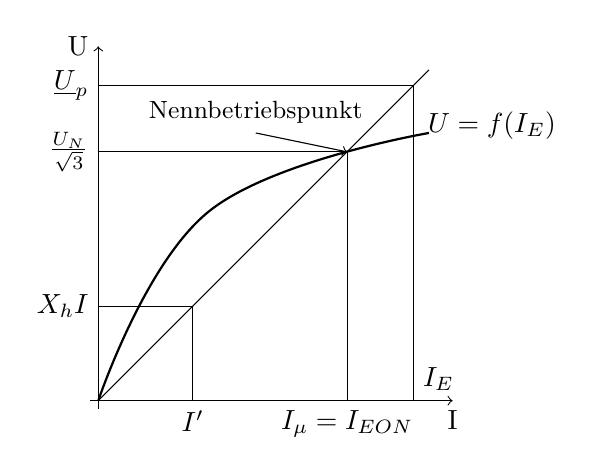
\begin{tikzpicture}
 	\draw[->] (-0.1,0) -- +(4.6,0) node[below] {I};
 	\draw[->] (0,-0.1) -- +(0,4.6) node[left]{U};
 	\draw (0,0) -- +(4.2,4.2);
	\draw[thick]  plot[smooth, tension=.7] coordinates {(0,0) (1.4,2.4) (4.2,3.4)};
	\draw (5,3.5) node[] {$U = f(I_E)$};
	
	\draw (1.2,0) node[below] {$I'$}
		-- ++(0,1.2) 
		-- ++(-1.2,0) node[left] {$X_h I$};
	\draw (3.16,0) node[below] {$I_\mu = I_{EON}$}
		-- ++(0,3.16) 
		-- ++(-3.16,0) node[left] {$\frac{U_N}{\sqrt{3}}$};
	\draw (4,0) node[above right] {$I_E$}
		-- ++(0,4) 
		-- ++(-4,0) node[left] {$\underline{U}_p$};
	\draw[<-] (3.16,3.16) -- (2,3.4) node[above]{\small{Nennbetriebspunkt}};
\end{tikzpicture}}
	    		\caption{Im Betriebspunkt linearisierte Leerlaufgerade}
	    	\end{subfigure}
	    	\begin{subfigure}[t]{0.45\textwidth}
	    		\centering
	    		\adjustbox{scale=0.8}{\begin{tikzpicture}
 	\draw[->] (-0.1,0) -- +(4.6,0) node[below] {$i_E$};
 	\draw[->] (0,-0.1) -- +(0,4.6) node[left]{$\frac{I_k}{I_N}$};
 	\draw (0,0) -- +(4.2,4.2);
	
	\draw (1.8,0) node[below] {$1$}
		-- ++(0,1.8) 
		-- ++(-1.8,0) node[left] {$i_{k0}$};
	\draw (3.6,0) node[below] {$i_{Ek}$}
		-- ++(0,3.6) 
		-- ++(-3.6,0) node[left] {$1$};
\end{tikzpicture}}
	    		\caption{Kurzschlussgerade}
	        \end{subfigure}
	        \caption{Kurven in den Verschiedenen Betriebsarten}
	        \label{fig:betriebsverhalten}
    	\end{figure}
    	
    	\begin{tabular}{ l l p{9cm} }
    		\textbf{Leerlauf}
    		& $I_E = \frac{U_P \cdot \sqrt{3} \cdot I_{E0N}}{U_N}$ 
    		& Die Formel ist für die liniarisierte Gerade \newline
    		  $I_E: $Erregerstrom \newline
    		  $U_P: $verkettete Nennspannung des DS- Netzes\newline
    		  $I_{E0N}:$Leerlauferregerstrom für Nennspannung
    		\\
    		\textbf{Kurzschluss} 
    		& $X_d=\frac{U_P}{I_{K0}}$
    		& Gilt unter Vernachlässigung des Wicklungswiderstand \newline
    		  Die Kurzschlussgerade ist linear
    		\\
    	\end{tabular} 
    	

    \subsubsection{Inselbetrieb}
        \begin{minipage}{10cm}
            \abb{images/Belastungskennlinie_DSM.png}{9cm}{Belastungskennlinie bei konst. Erregerstrom}
        \end{minipage}
        \begin{minipage}{6cm}
            \abb{images/Regulierungslinie_DSM.png}{6cm}{Regulierungskennlinie für konst. $U_{Kl}$}
        \end{minipage} \\
        Die Klemmenspannung nimmt bei kapazitiven Lasten zu, bei induktiven stark ab. Für eine konstante $U_{Kl}$ muss der Erregerstrom wie die Regulierungskennlinie angepasst werden.

    \subsubsection{Netzbetrieb}
        Im Netzbetrieb wird die Frequenz, Klemmenspannung, Umlaufsinn und Phasenlage vom Netz vorgegeben. Das heisst bevor man mit einer DSM ans Netz will, muss man sie so synchronisieren, dass alle jene Parameter mit dem Netz überreinstimmen. Sind die Maschine und Netz synchronisiert und zusammengeschaltet, kann mit Hilfe von $I_E$ und der mechanischen Leistung der Blindstromanteil eingestellt werden: \\
        \begin{minipage}{8.2cm}
            \abb{images/Ortskurve_DSM.png}{8cm}{Ortskurve einer DSM im starren Netz}
        \end{minipage}
        \begin{minipage}{9.7cm}
            \begin{itemize}
                \item Da $U_{Kl} = U_1$ konstant ist, ist der Ursprung des Zeigers $\frac{j \cdot U_p}{X_d}$ immer am gleichen Ort. 
                \item Mit dem Erregerstrom kann man die Länge des Zeigers $\frac{j \cdot U_p}{X_d}$ einstellen.
                \item Die mechanische Leistung ist proportional zum Abstand der Zeigerspitze zur Imaginärachse.
                \item Die Blindleistung ist proportional zum Abstand  der Zeigerspitze zur Reelenachse.
                \item Ist nun die mechanische Leistung konstant und man ändert den Erregerstrom, so wandert die Zeiger auf einer Linie parallel zur Imag-Achse hin und her.
                \item Überschreitet der Zeiger die Stabilitätslinie, schlipft der Läufer durchund es gibt grosse Lärm- und Wärmeentwicklung, da die mechanische Leistung zu gross wird für den Erregerstrom.
                \item Bleibt der Erregerstrom konstant und die mechanische Leistung ändert sich, so wandert der Zeiger auf dem Kreis um (0,$\frac{U_Kl}{j \cdot X_d}$). Jedoch wiederum nur bis zur Stabilitätsgrenze, da dort die Wirkleistung für diesen Erregerstrom maximal ist.
            \end{itemize}
        \end{minipage}
        \\ \\ \\
        $$ U_P = \sqrt{\frac{U^2_{Netz}}{3} + X_d^2 \cdot I^2 + 2 \cdot \frac{U_{Netz}}{\sqrt{3}}\cdot X_d \cdot I \cdot \sin(\varphi)} $$